\section{Context and Motivation}

\subsection{Context} 

\acrfull{das} is a technology that enables real-time acoustic sensing along fiber-optic cables by analyzing Rayleigh backscattering in the optical fiber \cite{shang2016optical}. The system sends light pulses through the fiber and detects the light that returns after being backscattered from small imperfections along the fiber's length, as shown in Figure \ref{fig:das-fig}. By analyzing changes in the backscattered light, \acrshort{das} can detect and localize acoustic disturbances along the entire fiber. This technology has gained more recognition within the last decade, and due to its high sensitivity, these systems can detect subtle environmental changes and anomalies. Analyzing these irregularities is a common and crucial task in various fields, and it can be applied to tasks such as landslide and earthquake detection as well as railroad and maritime monitoring. The ability to process and interpret \acrshort{das} data effectively and efficiently is essential for extracting meaningful insights from these complex measurements in real-time environments. \\

\begin{figure}[htbp]
    \centering
    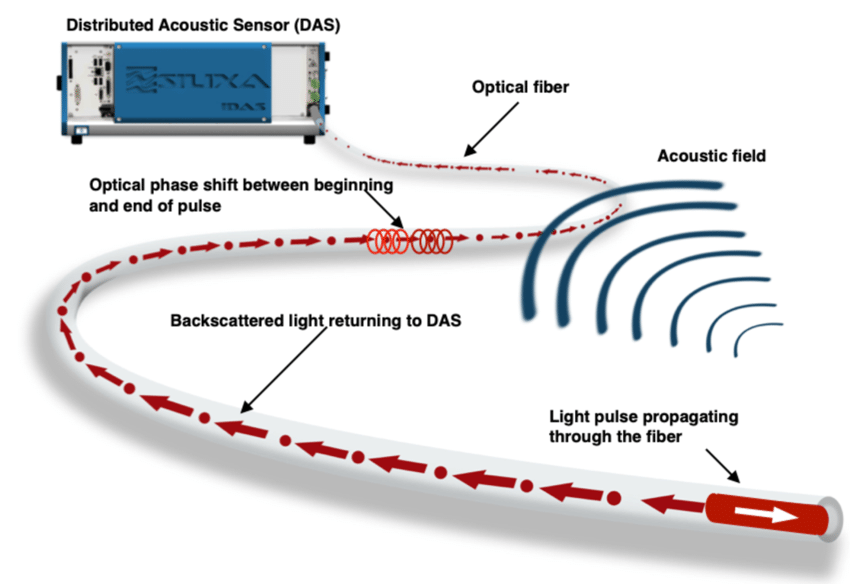
\includegraphics[width=0.7\linewidth]{figures/das.png}
    \caption{Showcase of how \acrshort{das} signals are recorded\footnotemark}
    \label{fig:das-fig}
\end{figure}

\footnotetext{\label{fn:das-image-source}Image source: \url{https://www.researchgate.net/publication/344127365/figure/fig1/AS:1073735670960128@1633009941244/Operation-principle-of-Distributed-Acoustic-Sensing-DAS.png}}

Anomaly detection is the process of finding outliers in datasets that differs greatly from others \cite{anomaly}. In the context of \acrshort{das} data, the objective is to find groups of irregular sensor signals that differs greatly from the rest of the recorded data. 
Several supervised \acrfull{ml} algorithms such as K-MEANS \cite{hartigan1979k} DBSCAN \cite{ester1996density} have been quite popular for anomaly detection on \acrshort{das} data. Over the last decade, a popular modification to the DBSCAN algorithm, HDBSCAN \cite{rahman2016hdbscandensitybasedclustering}, has also shown prowess in clustering-based anomaly detection \cite{ariyaluran2022clustering}. However, these methods often require manual feature engineering, require labeled datasets, or do not scale to large datasets CITE.  \\
In later years, unsupervised \acrshort{ai} and \acrshort{ml} models have been utilized for analyzing \acrshort{das} data. Compared to their supervised alternatives, unsupervised deep neural networks do not require manual labeling. They're therefore not prone to the same issues, such as detecting unlabeled anomalies \cite{wei2022lstmautoencoder, srivastava2016unsupervised} compared to their supervised alternatives. This makes them particulary good for analyzing \acrshort{das} data, where all kinds of anomalies can occur. 
Among unsupervised deep learning models, autoencoders have been proved efficient for analyzing \acrshort{das} data CITE. Autoencoders are neural networks designed to learn efficient data codings in an unsupervised manner, making them well-suited for dimensionality reduction and anomaly detection in complex, high-dimensional datasets like those produced by \acrshort{das} systems.

\subsection{Motivating challenges}

\acrshort{cgf} currently expends considerable time and resources on processing and analyzing \acrshort{das} data. Existing tools are predominantly sequential, failing to leverage parallelization, and often load entire datasets into memory. This approach severely limits the volume of data that can be processed simultaneously, leading to inefficiencies in handling the large-scale datasets typical in \acrshort{das} experiments. 

While languages such as Python and Matlab are commonly used at \acrshort{cgf} due to familiarity, these languages may not be optimal for data-intensive applications without integrating lower-level languages like C. Julia, a relatively new language designed for both data science and \acrfull{hpc}, offers a promising alternative. Its potential for developing scalable \acrshort{das} processing applications remains largely unexplored, despite its suitability for handling large-scale scientific computations efficiently. 

Furthermore, although numerous autoencoder models exist for \acrshort{das} data analysis, many fail to prioritize memory efficiency or computational complexity. This oversight is particularly problematic for real-time applications, where rapid processing of large data volumes is crucial. There is a clear need for more models that balance analytical power with computational efficiency. 

The \acrshort{das} field suffers from a notable lack of \acrfull{foss} datasets and unsupervised \acrshort{ai} models. This is partly due to \acrshort{das} often recording confidential data. This scarcity hinders research progress and reproducibility. Developing open-source programs for training autoencoders on \acrshort{das} data could significantly advance the field by providing accessible tools and benchmarks for the field.  

Despite the promising potential of unsupervised \acrshort{ai} algorithms for anomaly detection in \acrshort{das} data, their application at \acrshort{cgf} remains limited. This represents a missed opportunity for enhancing the efficiency and accuracy of \acrshort{das} data analysis, particularly in identifying complex patterns and anomalies that traditional methods might overlook.

Addressing these challenges could substantially improve the processing and analysis of \acrshort{das} data, leading to more efficient utilization of resources, enhanced real-time capabilities, and broader accessibility of advanced analytical tools in the field.

